\documentclass{beamer}
\usepackage{url}
\usepackage{ragged2e}
\usetheme{metropolis}

\title{Writing with NAO}
\author{Adrien Bardes, Marius Dufraisse, Pierre Guetschel, Mengda Li}
%\institute{ENS Paris-Saclay}

\titlegraphic{
\includegraphics[scale = 0.2]{logo.png}}
\begin{document}

\frame{\titlepage}

\begin{frame}{Goal of our project}
We want to make our robot NAO write!
\medskip

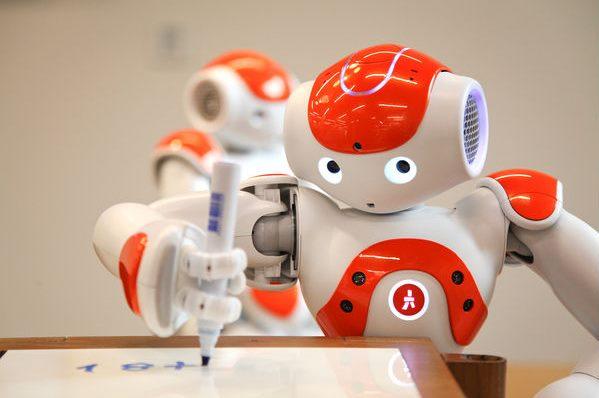
\includegraphics[scale = 0.7]{NAO_writes.jpg}\cite{1}
\end{frame}

\begin{frame}{Methodology}
\tableofcontents
\end{frame}

\section{Analysis of handwriting and extraction of trajectory function}
\begin{frame}{trajectory function}

We formalize what we want to write by a trajectory function.
\bigskip

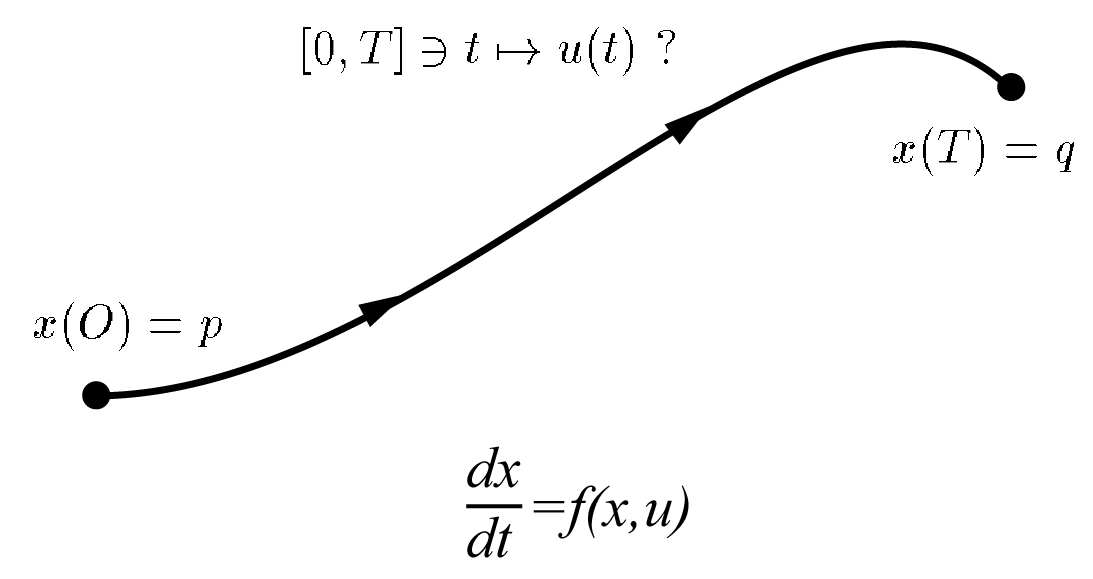
\includegraphics[scale = 0.3]{planning.jpg}\cite{2}
\end{frame}
\section{Inverse kinematics}


\begin{frame}{approching the goal trajectory}

We approach this goal trajectory by solving a sequence of optimization problem: minimizing the errors betwenn the goal trajectory and the real trajectory.
\medskip

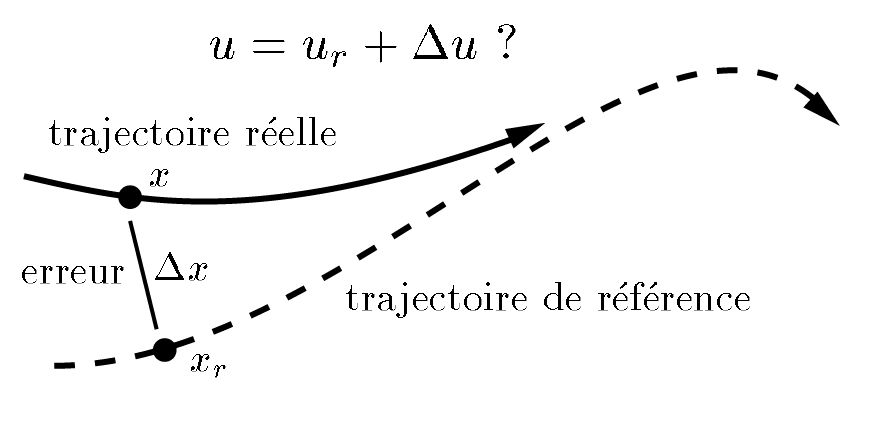
\includegraphics[scale = 0.4]{tracking.jpg}\cite{2}
\end{frame}

\begin{frame}[allowframebreaks]{modeling the coordinate system}

\begin{columns}
\begin{column}{0.5\textwidth}
\justify
   The robot is a n-joint system. 
   
   We find the position of end-effector (the pen) by composing a sequence of \emph{change of coordinates}.
\end{column}
\begin{column}{0.5\textwidth}  %%<--- here
    \begin{center}
     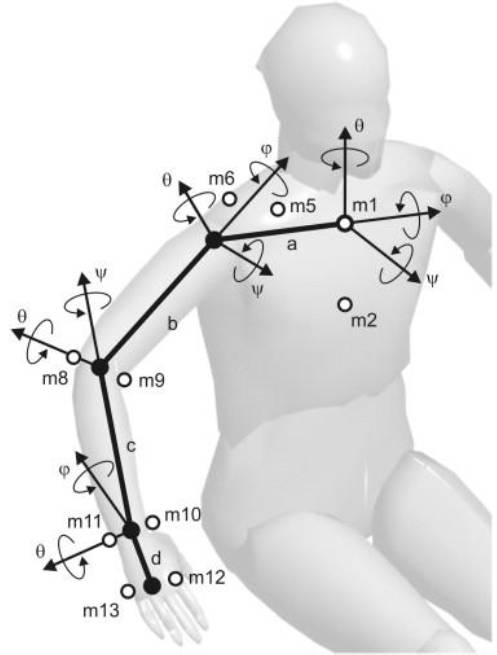
\includegraphics[scale = 0.35]{arm.jpg}\cite{3}
     \end{center}
\end{column}
\end{columns}


%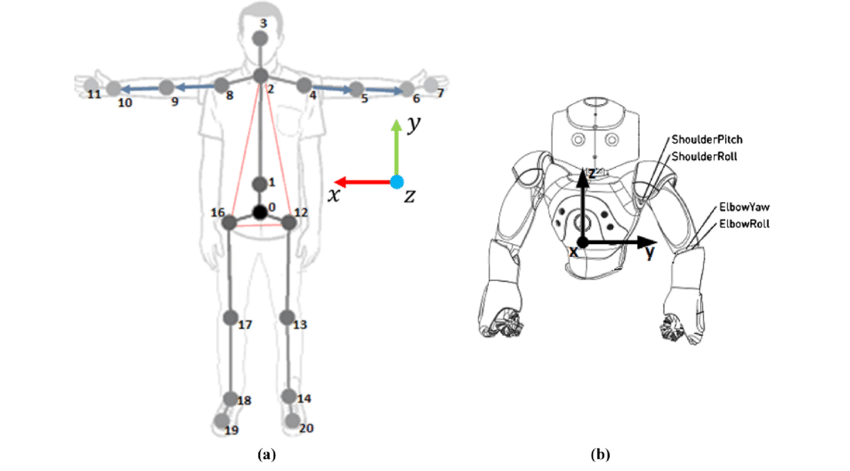
\includegraphics[scale = 0.35]{coordinate.png}\cite{3}

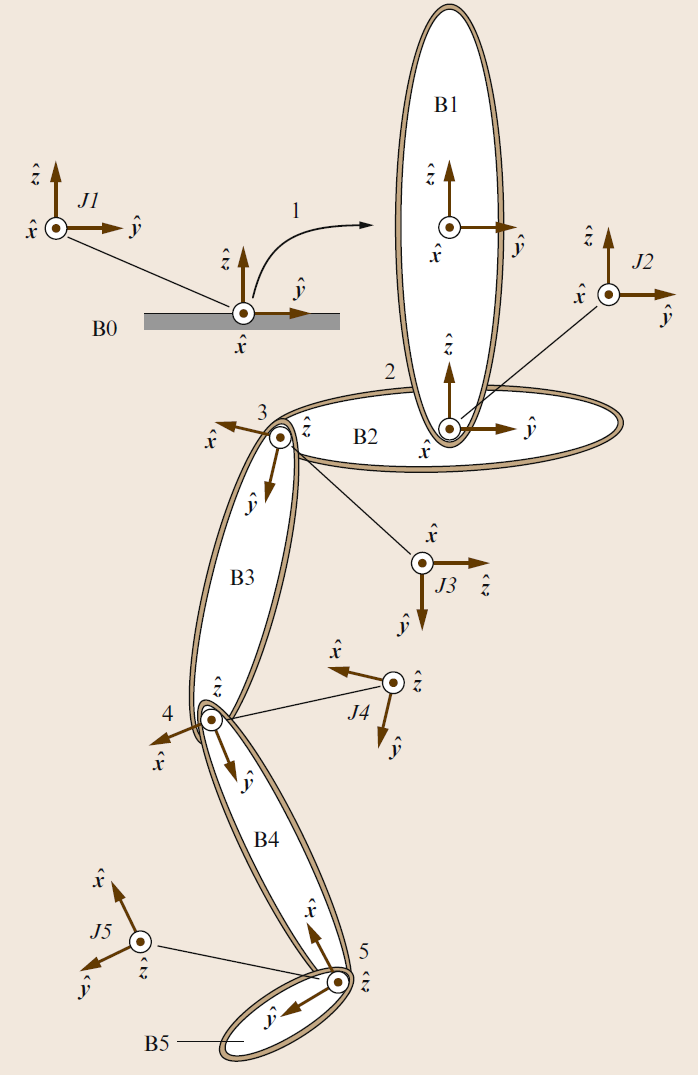
\includegraphics[scale = 0.3]{joints.png}\cite{4}
\end{frame}

\begin{frame}[allowframebreaks]{Bibliography}
\begin{thebibliography}{9}

\bibitem{1} 
NAO robot illustrating a TechCrunch article.
\path{https://www.robotlab.com/blog/nao-robot-illustrating-a-techcrunch-article}

\bibitem{2} 
Planification et suivi de trajectoires. 
\path{http://cas.ensmp.fr/~petit/smai/}
 
 \bibitem{3} 
\textit{Interfacing of Kinect Motion Sensor and NAO Humanoid Robot for Imitation Learning}. 
\path{https://www.youngscientistjournal.org/article/interfacing-of-kinect-motion-sensor-and-nao-humanoid-robot-for-imitation-learning}

\bibitem{y} 
Emrehan Yavşan, Ayşegül Uçar. 
\textit{Teaching human gestures to humanoid robots by using Kinect sensor}. 
\path{https://www.researchgate.net/publication/282829504_Teaching_human_gestures_to_humanoid_robots_by_using_Kinect_sensor}
 
\bibitem{4} 
Oussama Khatib.
\textit{Springer Handbook of Robotics}.
 Fig. 3.5
\end{thebibliography}

\end{frame}
\end{document}
